\documentclass[11pt]{beamer}
\usepackage{url,fancybox}
%\usepackage{pgfgantt}

\usepackage[utf8]{inputenc}
\parindent0pt
\parskip3pt

\newcommand{\Rahmen}[2]{
\setlength{\fboxsep}{12pt}\begin{center}
\shadowbox{\parbox{#1\textwidth}{\em #2}}\end{center}}

% Designelemente
\usetheme{Hannover}
\beamertemplatenavigationsymbolsempty
\title[The WUMM Project]{The WUMM Project\\ Semantic Data and Innovation
  Management}

\author[Hans-Gert Gr\"abe]{Prof. Hans-Gert Gräbe}
\institute{Institut f\"ur Informatik, Universit\"at Leipzig,\\
  \url{http://bis.informatik.uni-leipzig.de/HansGertGraebe/}}
\date{22. Mai 2019}
\begin{document}
\begin{frame}
\maketitle
\end{frame}

\begin{frame}{The WUMM-Project}
  WUMM forms the theoretical core of an innovation network in Middle Germany
  (Region Mitteldeutschland). Under such an open brand, we want to collect
  relevant concepts and materials and make them available to the general
  public.
  \begin{itemize}
  \item \url{http://leipzig-netz.de/index.php5/WUMM}\\ -- Wiki (in German)
  \item \url{https://wumm-project.github.io/}\\ -- github Pages (in English)
  \item \url{https://github.com/wumm-project/}\\ -- github organzational
    account
  \end{itemize}
\end{frame}


\begin{frame}{The Generic Innovation Problem}
Bild Business $\to$ Besseres Business

\end{frame}

\begin{frame}{Structured Innovation Approaches}
Bild konkrete versus abstrakte Ebene
\end{frame}

\begin{frame}{Design Thinking}
  \begin{center}
    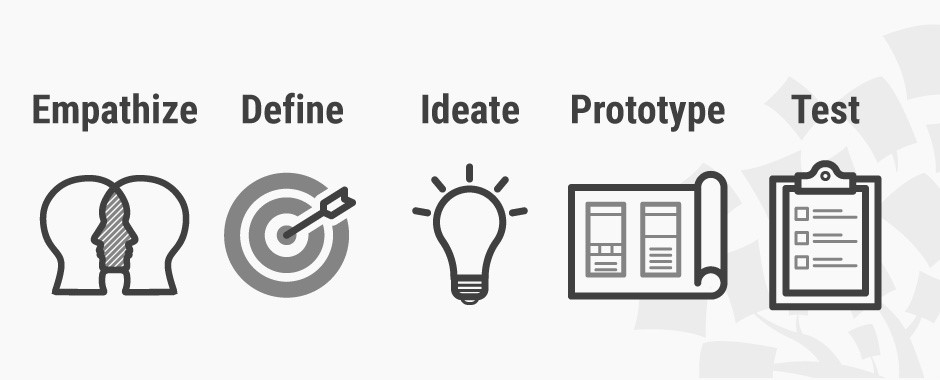
\includegraphics[width=.7\textwidth]{DesignThinking.jpg}
  \end{center}\scriptsize
    Design thinking is more than just a creative process. What was originally
    developed as an innovation method for products and services at Stanford is
    now becoming a whole new way of seeing people in relation to work,
    thinking about the concept of work, and asking how we live, learn and live
    in the 21st century want to work. The power of Design Thinking is to
    enable new and surprising forms of creative collaboration. We-intelligence
    is the new buzzword, collaboration becomes the basis for a new working
    consciousness.
    (\url{https://hpi.de/school-of-design-thinking/design-thinking.html})
\end{frame}

\begin{frame}{TRIZ and ARIZ-85C}

  
\end{frame}

\begin{frame}
  \begin{center}
    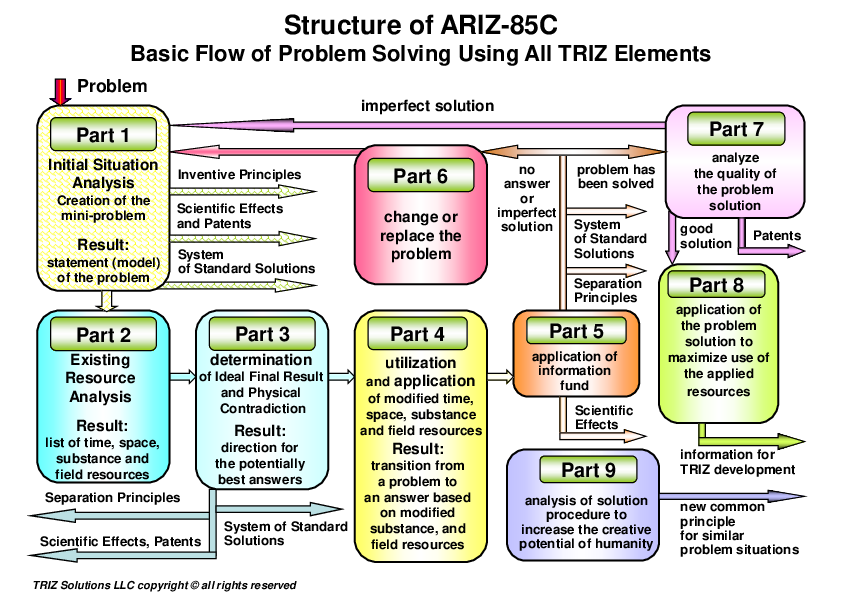
\includegraphics[width=\textwidth]{ARIZ-Workflow.png}
  \end{center}
\end{frame}


\end{document}
